\documentclass[tikz,border=4pt]{standalone}
% Shared pastel academic grammar for final-size technical-paper diagrams.
\usepackage[T1]{fontenc}
\usepackage{lmodern}
\usepackage{amsmath,amssymb}
\usepackage{xcolor}
\usepackage{tikz}
\usetikzlibrary{
  arrows.meta,
  backgrounds,
  calc,
  circuits.logic.US,
  decorations.pathreplacing,
  fit,
  matrix,
  patterns,
  positioning,
  shapes.geometric,
  shapes.symbols
}

\definecolor{ink}{RGB}{24,24,28}
\definecolor{midink}{RGB}{96,96,104}
\definecolor{paleink}{RGB}{184,184,190}
\definecolor{wash}{RGB}{241,240,237}
\definecolor{paper}{RGB}{255,255,253}
\definecolor{cyan}{RGB}{126,203,218}
\definecolor{cyanwash}{RGB}{211,238,242}
\definecolor{pink}{RGB}{235,139,158}
\definecolor{pinkwash}{RGB}{250,211,217}
\definecolor{purple}{RGB}{166,50,150}
\definecolor{purplewash}{RGB}{232,196,227}
\definecolor{gold}{RGB}{177,139,45}
\definecolor{goldwash}{RGB}{239,226,183}
\definecolor{slate}{RGB}{116,133,145}
\definecolor{slatewash}{RGB}{221,226,229}
\colorlet{muted}{midink}
\colorlet{rule}{paleink}
\colorlet{accent}{purple}
\colorlet{accentwash}{purplewash}
\colorlet{second}{cyan}
\colorlet{secondwash}{cyanwash}

\tikzset{
  every picture/.style={
    font=\rmfamily\footnotesize,
    text=ink,
    line cap=round,
    line join=round,
    >=Stealth
  },
  every node/.style={outer sep=0pt},
  panel mark/.style={font=\rmfamily\bfseries\footnotesize},
  primary/.style={font=\rmfamily\footnotesize},
  secondary/.style={font=\rmfamily\scriptsize,text=midink},
  signal name/.style={font=\ttfamily\footnotesize,anchor=east},
  scope trace/.style={draw=ink,line width=.62pt,line cap=butt,line join=miter},
  hairline/.style={draw=paleink,line width=.28pt,line cap=butt},
  dotted guide/.style={draw=midink,line width=.32pt,densely dotted},
  dashed scope/.style={draw=ink,line width=.45pt,dashed},
  transition/.style={-{Stealth[length=1.8mm,width=1.25mm]},draw=ink,line width=.58pt},
  transition label/.style={font=\rmfamily\scriptsize,fill=paper,inner sep=1.2pt},
  preedge/.style={circle,draw=ink,fill=paper,line width=.58pt,minimum size=8.2mm,inner sep=1pt},
  observed preedge/.style={preedge,fill=purplewash,double,double distance=1.15pt,line width=.62pt,minimum size=9.8mm},
  brace/.style={decorate,decoration={brace,mirror,amplitude=3pt},draw=ink,line width=.45pt},
  grid rule/.style={draw=slate,line width=.32pt,line cap=butt},
  outer rule/.style={draw=ink,line width=.82pt,line cap=butt,line join=miter},
  star mark/.style={star,star points=5,star point ratio=2.2,draw=ink,fill=purple,minimum size=5.1mm,inner sep=0pt},
  % Compatibility vocabulary used by the repository's other figures.
  flow/.style={-{Latex[length=4.5pt,width=3.2pt]},draw=ink,line width=.55pt},
  heavy flow/.style={-{Latex[length=5pt,width=3.6pt]},draw=ink,line width=.8pt},
  wire/.style={draw=ink,line width=.5pt},
  bus/.style={draw=ink,line width=1.05pt},
  guide/.style={draw=midink,line width=.4pt,dotted},
  alternate/.style={draw=ink,line width=.5pt,dashed},
  scope/.style={draw=ink,line width=.5pt,dashed,inner sep=6pt},
  block/.style={draw=ink,line width=.55pt,fill=paper,minimum height=8mm,inner xsep=5pt,inner ysep=4pt,align=center},
  operation/.style={block,fill=cyanwash,minimum width=17mm},
  register/.style={block,fill=paper,minimum width=16mm,minimum height=10mm},
  state/.style={circle,draw=ink,line width=.55pt,fill=cyanwash,minimum size=8mm,inner sep=1pt,align=center},
  terminal/.style={state,fill=purplewash,double,double distance=1.2pt,line width=.6pt},
  predicate/.style={diamond,aspect=1.8,draw=ink,line width=.55pt,fill=pinkwash,inner xsep=3pt,inner ysep=2pt,align=center},
  datum/.style={rectangle,draw=ink,line width=.5pt,fill=goldwash,minimum width=8mm,minimum height=6mm,inner sep=2pt,align=center},
  panel label/.style={font=\rmfamily\bfseries\footnotesize},
  local heading/.style={font=\rmfamily\bfseries\footnotesize},
  annotation/.style={font=\rmfamily\scriptsize,text=midink,align=center},
  heading/.style={font=\rmfamily\bfseries\small},
  subheading/.style={font=\rmfamily\bfseries\footnotesize},
  note/.style={font=\rmfamily\scriptsize,text=midink},
  label/.style={font=\rmfamily\bfseries\scriptsize},
  mono/.style={font=\ttfamily\footnotesize},
  tiny mono/.style={font=\ttfamily\scriptsize},
  count/.style={font=\rmfamily\bfseries\small},
  selected/.style={draw=ink,fill=purplewash,line width=.8pt},
  cell on/.style={fill=purple,draw=ink,line width=.3pt},
  cell off/.style={fill=paper,draw=paleink,line width=.3pt}
}

% Flat pastel facets and depth edges for restrained axonometric constructions.
\tikzset{
  cyan facet/.style={draw=ink,fill=cyanwash,line width=.5pt,line join=round},
  cyan side/.style={draw=ink,fill=cyan,line width=.5pt,line join=round},
  pink facet/.style={draw=ink,fill=pinkwash,line width=.5pt,line join=round},
  pink side/.style={draw=ink,fill=pink,line width=.5pt,line join=round},
  purple facet/.style={draw=ink,fill=purplewash,line width=.55pt,line join=round},
  purple side/.style={draw=ink,fill=purple,line width=.55pt,line join=round},
  gold facet/.style={draw=ink,fill=goldwash,line width=.5pt,line join=round},
  gold side/.style={draw=ink,fill=gold,line width=.5pt,line join=round},
  context facet/.style={draw=ink,fill=slatewash,line width=.45pt,line join=round},
  depth edge/.style={draw=midink,line width=.38pt},
  surface grid/.style={draw=slate,line width=.32pt},
  projection/.style={draw=midink,line width=.38pt,densely dashed},
  accent curve/.style={draw=purple,line width=1.05pt},
  cyan curve/.style={draw=cyan!70!ink,line width=.9pt},
  pink curve/.style={draw=pink!70!ink,line width=.9pt},
  gold curve/.style={draw=gold!80!ink,line width=.9pt}
}


\tikzset{
  observed frame/.style={
    draw=ink,
    fill=paper,
    line width=.62pt,
    rounded corners=2pt
  },
  phase band/.style={draw=none,fill opacity=.42},
  phase tag/.style={
    font=\rmfamily\bfseries\scriptsize,
    draw=ink,
    line width=.38pt,
    rounded corners=1.4pt,
    inner xsep=5pt,
    inner ysep=2.2pt
  },
  phase name/.style={
    font=\rmfamily\bfseries\scriptsize,
    text=ink,
    inner sep=0pt
  },
  model frame/.style={
    draw=purple!72!ink,
    fill=paper,
    line width=.55pt,
    dash pattern=on 4pt off 2.4pt,
    rounded corners=2pt
  },
  film state/.style={preedge,fill=paper,minimum size=8.4mm},
  film depth/.style={
    circle,
    draw=ink,
    fill=cyan,
    line width=.38pt,
    minimum size=8.4mm,
    inner sep=1pt
  },
  film terminal depth/.style={film depth,fill=purple},
  verdict callout/.style={
    purple facet,
    rounded corners=1.5pt,
    font=\rmfamily\scriptsize,
    align=center,
    inner xsep=5pt,
    inner ysep=2.5pt
  }
}

\begin{document}
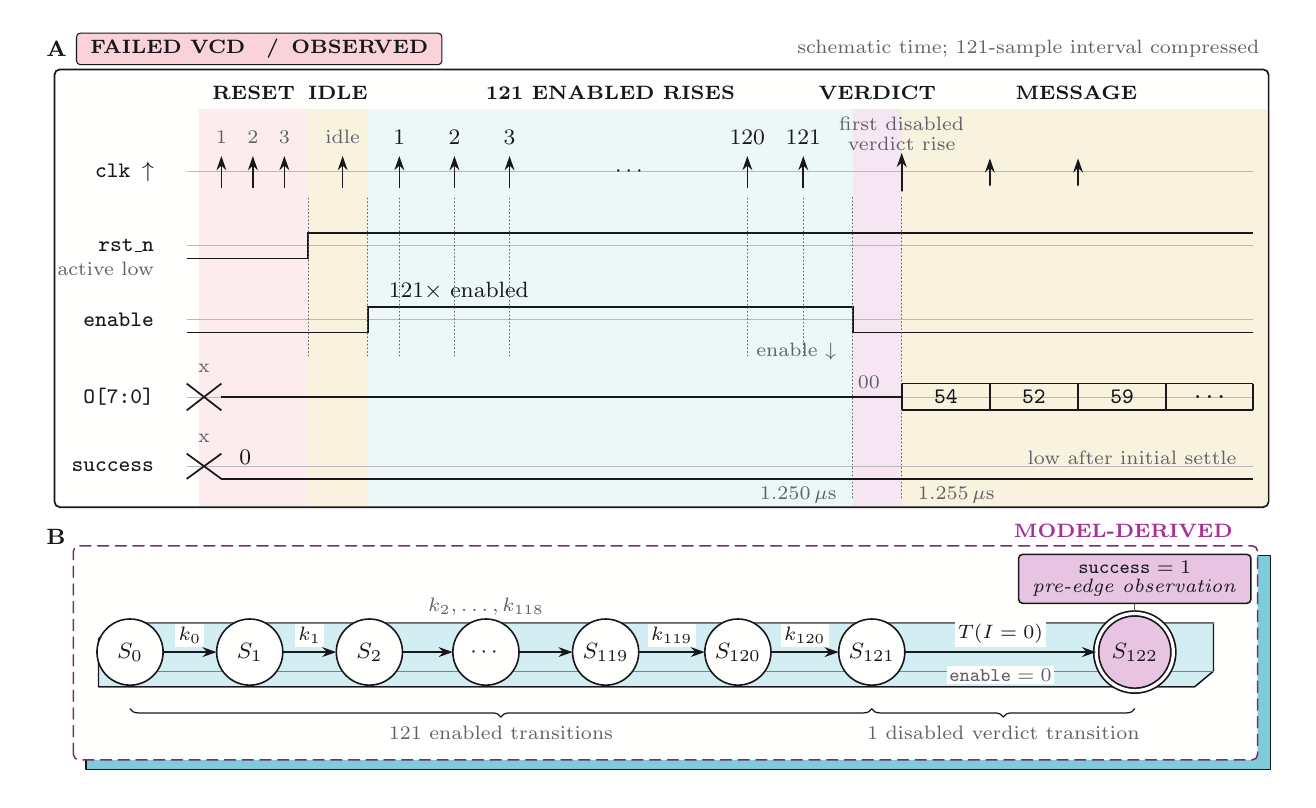
\begin{tikzpicture}
  \path[use as bounding box] (0,0) rectangle (16,9.55);

  % A. The observed scope remains orthographic; only semantic intervals are tinted.
  \node[panel mark,anchor=west] at (.12,9.28) {A};
  \node[phase tag,fill=pinkwash,anchor=west] at (.62,9.28)
    {FAILED VCD \enspace/\enspace OBSERVED};
  \node[secondary,anchor=east] at (15.76,9.28)
    {schematic time; 121-sample interval compressed};

  \path[observed frame] (.34,3.46) rectangle (15.76,9.02);
  \begin{scope}
    \clip[rounded corners=2pt] (.35,3.47) rectangle (15.75,9.01);
    \path[phase band,fill=pinkwash] (2.18,3.47) rectangle (3.56,8.52);
    \path[phase band,fill=goldwash] (3.56,3.47) rectangle (4.32,8.52);
    \path[phase band,fill=cyanwash] (4.32,3.47) rectangle (10.48,8.52);
    \path[phase band,fill=purplewash] (10.48,3.47) rectangle (11.10,8.52);
    \path[phase band,fill=goldwash] (11.10,3.47) rectangle (15.75,8.52);
  \end{scope}

  \node[phase name] at (2.87,8.72) {RESET};
  \node[phase name] at (3.94,8.72) {IDLE};
  \node[phase name] at (7.40,8.72) {121 ENABLED RISES};
  \node[phase name] at (10.79,8.72) {VERDICT};
  \node[phase name] at (13.32,8.72) {MESSAGE};

  \foreach \y/\name in {
    7.72/{clk $\uparrow$},
    6.78/{rst\_n},
    5.84/{enable},
    4.86/{O[7:0]},
    3.98/{success}
  }{
    \node[signal name] at (1.72,\y) {\name};
    \draw[hairline] (2.02,\y) -- (15.56,\y);
  }
  \node[secondary,anchor=east] at (1.72,6.49) {active low};

  % Exactly three reset rises, one idle rise, and selected landmarks in 121 rises.
  \foreach \x/\n in {2.46/1,2.86/2,3.26/3}{
    \draw[transition] (\x,7.52) -- (\x,7.92);
    \node[secondary] at (\x,8.16) {\n};
  }
  \draw[transition] (4.00,7.52) -- (4.00,7.92);
  \node[secondary] at (4.00,8.16) {idle};

  \foreach \x/\n in {4.72/1,5.42/2,6.12/3,9.14/120,9.85/121}{
    \draw[transition] (\x,7.52) -- (\x,7.92);
    \node[primary] at (\x,8.16) {\n};
  }
  \node[primary] at (7.66,7.72) {$\cdots$};

  \draw[transition,line width=.82pt] (11.10,7.48) -- (11.10,7.96);
  \node[secondary,align=center] at (11.10,8.20)
    {first disabled\\[-.3mm]verdict rise};
  \foreach \x in {12.22,13.34}{
    \draw[transition] (\x,7.55) -- (\x,7.89);
  }

  % Reset and enable are exact step traces, not perspective projections.
  \draw[scope trace]
    (2.02,6.62) -- (3.56,6.62) -- (3.56,6.94) -- (15.56,6.94);
  \draw[scope trace]
    (2.02,5.68) -- (4.32,5.68) -- (4.32,6.00) --
    (10.48,6.00) -- (10.48,5.68) -- (15.56,5.68);
  \node[primary,anchor=west] at (4.47,6.20) {$121\times$ enabled};

  \foreach \x in {3.56,4.32,4.72,5.42,6.12,9.14,9.85}{
    \draw[dotted guide] (\x,5.38) -- (\x,7.42);
  }
  \draw[dotted guide] (10.48,3.58) -- (10.48,7.42);
  \draw[dotted guide] (11.10,3.58) -- (11.10,7.42);
  \node[secondary,anchor=east] at (10.39,5.44) {enable $\downarrow$};

  % The byte bus has an initial X interval and changes first at the verdict rise.
  \draw[scope trace] (2.02,4.69) -- (2.46,5.03);
  \draw[scope trace] (2.02,5.03) -- (2.46,4.69);
  \node[secondary] at (2.24,5.23) {x};
  \draw[scope trace] (2.46,4.86) -- (11.10,4.86);
  \node[secondary,anchor=east] at (10.94,5.05) {00};
  \foreach \xa/\xb/\value in {
    11.10/12.22/54,
    12.22/13.34/52,
    13.34/14.46/59,
    14.46/15.56/{\ldots}
  }{
    \draw[scope trace] (\xa,4.69) -- (\xb,4.69);
    \draw[scope trace] (\xa,5.03) -- (\xb,5.03);
    \draw[scope trace] (\xa,4.69) -- (\xa,5.03);
    \node[primary] at ({(\xa+\xb)/2},4.86) {\texttt{\value}};
  }
  \draw[scope trace] (15.56,4.69) -- (15.56,5.03);

  % This failed run also has an initial X interval, then success stays low.
  \draw[scope trace] (2.02,3.82) -- (2.46,4.14);
  \draw[scope trace] (2.02,4.14) -- (2.46,3.82);
  \node[secondary] at (2.24,4.34) {x};
  \draw[scope trace,line width=.78pt] (2.46,3.82) -- (15.56,3.82);
  \node[primary,anchor=west] at (2.57,4.09) {$0$};
  \node[secondary,anchor=east] at (15.47,4.09) {low after initial settle};
  \node[secondary,anchor=east] at (10.39,3.61) {$1.250\,\mu\mathrm{s}$};
  \node[secondary,anchor=west] at (11.19,3.61) {$1.255\,\mu\mathrm{s}$};

  % B. A separate layered filmstrip: symbolic model, never part of the VCD.
  \node[panel mark,anchor=west] at (.12,3.08) {B};
  \path[cyan side] (.74,.13) rectangle (15.78,2.85);
  \path[model frame] (.58,.25) rectangle (15.62,2.97);
  \node[font=\rmfamily\bfseries\scriptsize,text=purple,anchor=east]
    at (15.42,3.16)
    {MODEL-DERIVED};

  % A shallow axonometric ribbon and offset state discs provide restrained depth.
  \path[cyan side]
    (.90,1.18) -- (14.82,1.18) -- (15.06,1.38) -- (1.14,1.38) -- cycle;
  \path[cyan facet,fill=cyanwash]
    (.90,1.18) -- (14.82,1.18) -- (15.06,1.38) -- (15.06,1.99) --
    (1.14,1.99) -- (.90,1.79) -- cycle;
  \draw[surface grid] (1.14,1.38) -- (15.06,1.38);
  \draw[surface grid] (1.14,1.99) -- (15.06,1.99);

  \node[film state] (s0) at (1.30,1.62) {$S_0$};
  \node[film state] (s1) at (2.82,1.62) {$S_1$};
  \node[film state] (s2) at (4.34,1.62) {$S_2$};
  \node[film state] (sdots) at (5.82,1.62) {$\cdots$};
  \node[film state] (s119) at (7.34,1.62) {$S_{119}$};
  \node[film state] (s120) at (9.02,1.62) {$S_{120}$};
  \node[film state] (s121) at (10.72,1.62) {$S_{121}$};
  \node[observed preedge] (s122) at (14.06,1.62) {$S_{122}$};

  \draw[transition] (s0) -- node[transition label,above=2pt] {$k_0$} (s1);
  \draw[transition] (s1) -- node[transition label,above=2pt] {$k_1$} (s2);
  \draw[transition] (s2) -- (sdots);
  \draw[transition] (sdots) -- (s119);
  \node[secondary,fill=paper,inner sep=1pt] at (5.82,2.20)
    {$k_2,\ldots,k_{118}$};
  \draw[transition] (s119) --
    node[transition label,above=2pt] {$k_{119}$} (s120);
  \draw[transition] (s120) --
    node[transition label,above=2pt] {$k_{120}$} (s121);
  \draw[transition,line width=.82pt] (s121) --
    node[transition label,above=2pt] {$T(I=0)$}
    node[secondary,below=5pt,fill=paper,inner sep=1pt] {$\mathtt{enable}=0$}
    (s122);

  \draw[brace] (1.30,.90) -- (10.72,.90)
    node[midway,below=3pt,secondary] {$121$ enabled transitions};
  \draw[brace] (10.72,.90) -- (14.06,.90)
    node[midway,below=3pt,secondary] {$1$ disabled verdict transition};

  \draw[projection] (14.06,2.13) -- (14.06,2.34);
  \node[verdict callout] at (14.06,2.55)
    {$\mathtt{success}=1$\\[-.4mm]\textit{pre-edge observation}};
\end{tikzpicture}
\end{document}
